\documentclass[12pt]{extarticle}
\usepackage[utf8]{inputenc}
\usepackage{cite}
\usepackage{graphicx}
\usepackage{subfig}

\graphicspath{ {/home/patrick/Pictures/} }
\usepackage{setspace}
\usepackage{amsmath}
\usepackage{indentfirst}
\setlength{\parskip}{10pt}
\title{Sequence to Sequence Modelling}
\author{Patrick Kahardipraja}
\date{September 2019}
\onehalfspacing

\begin{document}
% Make essay with style of literature review and blogposts

\maketitle
% Notes to remember: explain RNN and LSTM a bit?
% Problem of statistical machine translation?
% Applying seq2seq to many languages?
% Find seq2seq literature review
% Explain distributional representation?
% Tell about Google NMT?
% encoder - decoder
% transformer
% FOCUS ON DEVELOPMENT OF SEQ2SEQ OVER TIME AND HOW IT CHANGES
% Recent Advances: Facebook - Phrase-Based & Neural Unsupervised Machine Translation -> discuss that smt is not dead
% Cloze task and permutation LM as alternative to decoder LM?
% Change notation for probability!!

Mapping of a sequence to another sequence is an important paradigm because of the vast amount of problems that can be formulated in this manner. For instance, in automatic speech recognition (ASR), chunks of speech signals can be mapped to sequence of phonemes while in machine translation, a sequence of words in one language can be mapped to another language. Interestingly, many other tasks such as text summarization, question answering, and image caption generation can be phrased as a sequence to sequence problem. In this paper-style essay, I will attempt to distill how sequence to sequence learning works and the motivation behind it, with a particular focus on machine translation.


\section*{Introduction}

%Brief about SMT..(Prior to NMT)NN dead in 1990s. Resurgence of Deep Neural Networks (DNNs) in the last few years have been attributed to gpu power and availability of good dataset (ImageNet). Equipped with the capability to learn features automatically with multiple levels of representation, DNNs are already proven to achieve excellent performance on task such as object recognition (AlexNet). However, although powerful.. 

Prior to neural machine translation (NMT), phrase-based stastistical machine translation (SMT) systems are widely used as it offers reliable performance. Despite its success, most of them are extremely complex and require a huge amount of effort, as it is often tailored to a specific language pair and do not generalize well to another languages. In a phrase-based SMT system, a lot of feature engineering are required in order to capture a specific language phenomena, which prompt researchers to explore another approach. Furthermore, phrase-based systems still experience difficulty in capturing long-term dependencies.

The resurgence of deep neural networks (DNNs) in early 2010s, thanks to faster, parallel computation using GPUs and availability of large and high-quality datasets, bring a new wave of enthusiasm in deep models. With the capability to learn features automatically with multiple, hierarchical representation, DNNs achieve excellent performance on difficult tasks in computer vision [AlexNet] and speech recognition []. Albeit powerful, DNNs has its own limitation, as it requires input and output vectors with a fixed dimension and thus not suitable for sequence to sequence problem whose lengths are unknown beforehand. In addition, DNNs also do not generalize well across temporal patterns, because each neuron has its own specific connection and as a result, a single pattern may look totally different at different timesteps.

The natural remedy for this problem is to look onto recurrent neural networks (RNNs), as it allows operations over sequences of vectors. However, mapping using RNNs typically have one-to-one correspondence between the input vectors and the output vectors. It also has another problem, as the input and output sequences can have different lengths and non-monotonic alignments. Standard RNN architecture is also not reliable for learning long-range dependencies due to the vanishing gradient problem. This issue is addressed by Sutskever et al. [Seq2Seq], where they introduce a novel and straightforward method to solve general sequence to sequence mapping using Long-Short Term Memory (LSTM) architecture. With the success of sequence to sequence learning in machine translation tasks, research in neural machine translation continue to thrive, eventually resulting in many significant improvements such as attention mechanism [Bahdanau] and subword units to deal with rare words [WordPiece]. But, before delving in too deep, I will give some brief insight into the mechanism behind RNN and LSTM in the next section. 
%followed by?

\section*{Recurrent Neural Networks} % Discuss variants of RNN, LSTM, LSTM highway, GRU?

Recurrent neural networks [Rumelhart] are type of neural network that is able to process arbitrary sequential input via combination of its internal state and input vector. At every timestep $t$, the hidden state vector $h_{t}$ is overwritten as a function of the hidden state at the previous timestep $h_{t-1}$ and the current input vector $x_{t}$. The input vector $x_{t}$ itself could be a representation of $t$-th word in a sentence, which is usually obtained using pre-trained word embeddings [GloVe, Word2Vec, ElMo]. The hidden state of RNNs can be perceived as a memory with a fixed dimensionality that can be tuned, containing distributed representation of the processed input sequence up to time $t$.

In a RNN, the forward step function consists of an affine transformation followed by a non-linear activation function. The hidden state then can be used to make predictions:
\begin{align}
h_{t} &= a(W^{(x)}x_{t} + W^{(h)}h_{t-1} + b_{h})\\
y_{t} &= g(W^{(y)}h_{t} + b_{y}) 
\end{align}
where in a typical application, $a$ is the hyperbolic tangent function and $g$ is the softmax function.

Although proven to be effective, RNN still has its own shortcoming. The main problem with RNN is that during training, magnitude of gradient can get weaker or stronger exponentially when backpropagating the error through time, especially with long sequences [Hochreiter, Bengio]. This phenomena is called vanishing or exploding gradient problem, which causes RNN model to experience difficulty when handling "long-term dependencies" that occur in a sequence.

Long Short Term Memory (LSTM) architecture [Hochreiter and Schmidhuber] addresses the problem of "long-term dependencies" by integrating a memory cell that is capable to memorize state that span over long sequences of time. The memory cell is controlled by gates, which have the ability to regulate how much information are added or removed in the memory cell. This means that while in a RNN a completely new hidden state is computed at every new timestep, in LSTM the hidden state is not competely overwritten, and updated according to the memory cell. The architecture of both RNNs and LSTMs are depicted in Figure \ref{fig:rnn}.
\begin{figure}[ht]
\centering
\subfloat[RNN unit]{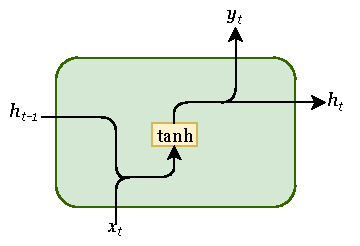
\includegraphics[scale=1.25]{rnn}} \\
\subfloat[LSTM unit, colah]{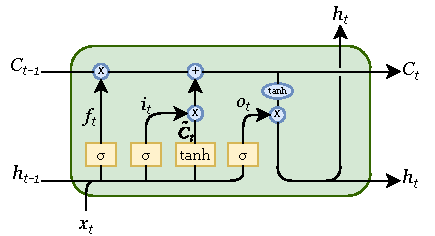
\includegraphics[scale=1.4]{lstm}}

\caption{Architecture of RNN (a) and LSTM (b)}
\label{fig:rnn}
\end{figure}

A LSTM unit consists of 3 gates (input gate $i_{t}$, forget gate $f_{t}$, output gate $o_{t}$), memory cell $C_{t}$ and hidden state $h_{t}$. In a high-level sense, the input gate decides how much and which values will be updated, the forget gate controls the amount of information to be forgotten in the previous memory cell, and the output gate decides the hidden state by filtering the internal memory cell for each timestep. Each gate produces vectors, where their values are between 0 (completely closed) and 1 (completely open) using the sigmoid activation function. 

The formula of LSTM is described with the following equations:
\begin{align}
i_{t} &= \sigma(W^{(i)}x_{t} + U^{(i)}h_{t-1} + b_{i}) \\
f_{t} &= \sigma(W^{(f)}x_{t} + U^{(f)}h_{t-1} + b_{f}) \\
o_{t} &= \sigma(W^{(o)}x_{t} + U^{(o)}h_{t-1} + b_{o}) \\
\tilde{C}_{t} &= \textnormal{tanh}(W^{(c)}x_{t} + U^{(c)}h_{t-1} + b_{c}) \\
C_{t} &= f_{t} \odot C_{t-1} + i_{t} \odot \tilde{C}_{t} \\
h_{t} &= o_{t} \odot \textnormal{tanh}(C_{t})
\end{align}
where $x_{t}$ is the input vector for timestep $t$, $\sigma$ is the sigmoid activation function and $\odot$ denotes the Hadamard product of matrices. 

\subsection*{Variants of LSTM}
%GRU, LSTM with peephole
Beside the standard LSTM architecture in literature that is introduced above, there also exist several popular variants which are commonly used. One of the variations which is introduced by [Gers, Schmidhueber] use "peephole connections". These connections allow the gates to look into the memory cell state in order to learn precise and stable timings. 

Other notable LSTM variants is the Gated Recurrent Unit (GRU), introduced by [Cho et al.]. Unlike LSTM, GRU is less complex and requires less computation. GRU only have 2 gates, the update gate that decides how much information will be transferred from previous and candidate hidden state to the current one and reset gate that controls to what extent the previous hidden state will affect the candidate hidden state. In this manner, the update gate can be thought as a combination of input and forget gates of LSTM unit. This architecture also merges the internal memory cell and hidden state of LSTM into a single hidden state.

% Add part for MT?Seems Cho et al. paper for GRU has a bit of reference for SMT
% Kalchbrenner and Cho 3 pg. max!!
\section*{Related Works}
The first model that is able to map a sentence into a vector and then to its translation is introduced by [Kalchbrenner et al.]. The model, which they called Recurrent Continuous Translation Models (RCTM), is composed of 2 separate parts: convolutional neural network (CNN) for modelling the source sentence as the encoder and recurrent neural network for translation generation as a language modelling task, conditioned on the source sentence as the decoder. With this approach, the encoder can capture all the information contained in the source word representations and create a representation of the source sentences. The representation for the source sentences also restraint the generation of the target words in the language modelling phase.
% How convolutional layers work, how RNN LM works. Explain 1d Conv in context of CSM.Advantage and disadvantage of RCTM. Explain Cho et al. model. Explain encoder-decoder from Kalchbrenner thesis

The Recurrent Continuous Translation Models estimate the probability distribution over the sentence in the target language given sentences in the source language. Suppose that there exist a target sentence $f = f_{1},f_{2},...,f_{m}$, which is a translation of source sentence $e = e_{1}, e_{2},...,e_{n}$. Then $p(f|e)$ can be obtained with the formula:
\begin{align} \label{eq:9}
p(f|e) = \prod_{i=1}^{m} p(f_{i}|f_{1:i-1}, e)
\end{align}

As can be seen in the formulation above, the model estimates $p(f|e)$ by calculating the conditional probability $p(f_{i}|f_{1:i-1}, e)$ for every translated word occuring at position $i$, given the preceding generated words $f_{1:i-1}$ in the target sentence and the source sentence $e$. Conditioning the translation model to the preceding target words also ensure that it incorporates the target language model [Kalchbrenner et al.].

In RCTM, prediction of the target sentence use a language model based on a recurrent neural network [Mikolov et al.]. The recurrent language model (RLM) predict the $i$-th word of the target sentence depending on all the previous generated words $f_{1:i-1}$, making no Markov assumption about the words dependencies in the target sentence. However, using the standard RNN architecture makes the prediction to be strongly affected by words close to $f_{i}$ and weakly influenced by long-range dependencies that occur in the target language due to the nature of RNN.

The RLM models probability of a sequence of words $f$ that occur in a language, which is denoted by $p(f)$. The equation for $p(f)$ is almost identical to Eq. \ref{eq:9} :
\begin{align}
p(f) = \prod_{i=1}^{m} p(f_{i}|f_{1:i-1})
\end{align}
It also contains a vocabulary $V$ for words $f_{i}$ of the language and 3 transformation matrices for input vocabulary $\textbf{I}$, recurrent transformation $\textbf{R}$ and output vocabulary transformation $\textbf{O}$. Each word $f_{k} \in V$ is distinguished by one-hot vector $v(f_{k})$. The computation then proceed as follows: 
\begin{align}
h_{1} &= g(\textbf{I} \cdot v(f_{1}) + b_{h}) \\
h_{i+1} &= g(\textbf{R} \cdot h_{i} + \textbf{I} \cdot v(f_{i+1}) + b_{h}) \\
o_{i+1} &= \textbf{O} \cdot h_{i} + b_{o}
\end{align}
and the probability distribution is obtained using the softmax function, 
\begin{align}
p(f_{i} = v | f_{1:i-1}) = \frac{\exp(o_{i,v})}{\sum_{v=1}^{V}\exp(o_{i,v})}
\end{align}
where $g$ is a nonlinearity and $\textbf{I} \cdot v(f_{i})$ is a continuous representation of word $f_{i}$.

There are 2 types of conditioning architecture in RCTM using CNN, using convolutional sentence model (CSM) and convolutional $n$-gram model (CGM). The CSM creates sentence representation in a bottom-up manner, using $n$-grams representations in the sentence itself. The hierarchical structure that is created by the model act quite similar like a parse tree in a implicit way. Using this type of structure, the model is able to capture the small, local representations in the lower layers of the model and more globally in the upper layers of the model as it spans more $n$-grams that comprise the sentence representations. This model also offers several advantages as it does not rely on a parse tree [Grefenstette 2011, Socher 2012]. As there exist many languages for which highly accurate and reliable parsers are not available, this model can still be robustly applied. Furthermore, the distribution of translation probability is learned by the model and does not depend on the chosen parse tree.

Using the continuous representations of words in the sentence, CSM models the representation of the sentence by applying sequence of one-dimensional convolution operations. The kernel of the convolutional layers is able to learn pattern within $n$-grams that convey syntactic, semantic or structural information relevant for constructing the sentence representation. After several convolution operations, the sentence vector representation $\textbf{e}$ is created at the topmost layer of the network for the source sentence $e$. This vector representation is then used in the RLM, after applying learned sentence transformation $\textbf{S}$. However, this model has a bias as the RLM tend to predict target sentences with shorter length. The sentence vector representation $\textbf{e}$ also constraint the target words, which is counterintuitive as it often occurs that the target translation has a strong dependencies on some parts of the source sentence and less on the other parts. In order to address these aspects, [Kalchbrenner et al.] also proposes the convolutional $n$-gram model as another conditioning architecture.

The CGM is a truncated version of the CSM, where the $n$-grams representation is extracted from a specific CSM layer for a chosen value of $n$. Using the $n$-grams representation of the source sentence $e$, the CGM can also be inverted to obtain representation for the target sentence $f$ with de-convolutional operation, where the length of the target sentence $m$ is estimated using Poisson distribution. This inverted CGM can also be thought as the truncated version of the inverted CSM for sentence length $m$. Before the inverted CGM unfolds the $n$-gram representation to a target sentence, a learned translation transformation $\textbf{T}$ is applied. The reconstructed vector for the source sentence representation is then added in an incremental manner to the corresponding hidden state $h_{i}$ in the RLM to predict the word $f_{i}$ in the target language. The issue that is addressed with the CGM model, where generation of the target words can now incorporate different parts of the reconstructed source sentence representation, is also later improved by [Bahdanau et al.], where they propose attention mechanism to learn soft-alignment between the source and target sentences.
% at end of CGM, connect problem of CSM with Bahdanau!!!

While the model proposed by [Kalchbrenner et al.] works quite well in for rescoring translation hypotheses from SMT system and computing perplexity of reference translations, using CNN as encoder means that the ordering of the words are not preserved. In an almost similar manner to this approach, [Cho et al.] attempt to map source sentence to a fixed vector representation then back to the target sentence, but with two RNNs as encoder and decoder. The encoder RNN reads each word in the source sentence sequentially until it reach the end of the sequence, which is marked by an end-of-sequence symbol. The hidden state of RNN after completely reading the source sentence is then encoded to a context vector $\textbf{c}$, which contains the summary of the whole source sentences. Consider source sentence $x$ with length $N$ and target sentence $y$ with length $M$. The encoder is formulated as follows:
\begin{align}
h_{t} &= RNN_{enc}(h_{t-1}, \textnormal{emb}(x_{t})) \\
\textbf{c} &= \textnormal{tanh}(\textbf{V}_{enc} \cdot h_{N})
\end{align}
where emb($x_{t}$) is a continuous representation of input word at timestep $t$ and $\textbf{V}_{enc}$ is a learned transformation for the encoder. 

On another part, the decoder RNN is a recurrent language model, conditioned on all the previous generated target words and the context vector $\textbf{c}$. It is computed as follows, where the decoder hidden state is initialized using the context vector:
\begin{align} 
h'_{0} &= \textnormal{tanh}(\textbf{V}_{dec} \cdot \textbf{c}) \\
h'_{t} &= RNN_{dec}(h'_{t-1}, \textnormal{emb}(y_{t-1}), \textbf{c}) 
\label{eq:18}
\end{align}
where $\textbf{V}_{dec}$ is a learned transformation for the decoder. The probability distribution of target words are obtained from a softmax function applied to the output of a feedforward neural network that consists of a single intermediate layer with maxout units [Goodfellow], using the decoder hidden state, context vector and target word generated from the previous timestep as inputs.
%generate output using DNN!!

For words representation, one-hot encoding is used to distinguish words in the vocabulary, which are then projected twice, yielding a 100-dimensional embedding for each word.
Both of the encoder and decoder use GRU instead of LSTM as it is easier to compute and implement. The encoder and decoder components of the model are then trained in an end-to-end fashion in order to estimate the conditional probability of the target sentence given the source sentence: 
\begin{align}
p(y|x) = \prod_{t=1}^{M} p(y_{t} | y_{t-1}, y_{t-2},...,y_{1}, \textbf{c}) \label{eq:19}
\end{align}
In their paper, they focus on integrating the RNN encoder-decoder pair for conventional phrase-based SMT system. The trained RNN encoder-decoder pair is used to rescore phrase pairs between the source and target sentences. This new score is then added to the existing phrase table and used as additional features in the log-linear model for the phrase-based SMT system. Furthermore, the model is also able to produce well-formed phrases in the target language independently without any influence from the actual phrase table.

% how they integrate enc-dec in smt system? what linguistic features do they learn?

\section*{Seq2Seq Model}
%Cho and Kalchbrenner didnt attempt direct translation. LSTM with multiple layers?
The works of [Kalchbrenner] and [Cho] however focus only on rescoring and not direct translation, although [Cho] mentions the possibility of replacing phrase table with phrases generated by the RNN encoder-decoder model. [Sutskever et al.] introduces a sequence-to-sequence model, often called "Seq2Seq", which achieves success to produce direct translation from English to French. The Seq2Seq model involves two RNNs as encoder and decoder, similar to [Cho].


The task of the encoder is to process the input sequence (source sentence in this case) in a sequential manner until its reaches the end-of-sentence (EOS) symbol to generate a fixed-dimensional context vector $\textbf{c}$ that represents the input sequence. It is also important to note that the encoder of Seq2Seq model processes input sequence in reverse. The idea behind reversing the input sequence is to reduce the "minimal time lag" [schmidhueber] problem. By doing this, the distance between first few words in the source and target languages are now much closer to each other, therefore making it easier for backpropagation to relate the source sentence and the target sentence. This method make it easier for the decoder to generate first few words correctly, and in turn improve the probability of generating the correct target translation. The illustration of the input sequence reversal is depicted on Fig..%Illustration

\newpage % buffer for images
The decoder architecture of the Seq2Seq model is almost similar to the decoder in the model proposed by [Cho et al.]. It is a recurrent language model, conditioned on all the target words that have been generated until the current timestep and the context vector $\textbf{c}$ that encapsulates all the information contained within the input sequence. The main difference between the Seq2Seq model and the RNN encoder-decoder model is that in Seq2Seq model, the context vector $\textbf{c}$ is only used for initializing the decoder hidden state whereas in the RNN encoder-decoder model, $\textbf{c}$ is used for decoder hidden state initialization and also for target words generation at all timestep, which is indicated in Eq. \ref{eq:18}. 

When the source sentence is already encoded into $\textbf{c}$ and the decoder is set up with the context vector, a special symbol is passed on to the decoder to mark the generation of the output sequence. In the paper, this is an EOS symbol that signifies the end of the input sequence. Afterwards, the decoder will continuously generate words in the target language until it generates the EOS symbol. The architecture of Seq2Seq model is depicted on Fig..
%Illustration of encoder and decoder model, with deep layers
%4 layers deep models, use lstm. paper that shows lstm is better than gru
% formula, beam search
% experiment in paper, model analysis pca
%teacher forcing?
\newpage
The encoder and decoder architecture of the Seq2Seq model use LSTM as it is capable of learning long range temporal dependencies. Compared to GRU, LSTM cells consistently performs better on language modelling [Jozefowicz et al. An Empirical Exploration of Recurrent Network Architectures] and machine translation tasks [Thang Luong Massive Exploration of NMT architectures]. The performance of LSTM can also be improved further by setting a large bias to the forget gate. To increase the model capacity, the implementation of Seq2Seq use deep LSTMs (4 layers in the paper) for the encoder and the decoder where the hidden state of encoder final layer at the last timestep is used as context vector $\textbf{c}$ to initialize the first layer of the decoder LSTM. Each additional layer of the deep LSTMs was also found to be able to reduce the perplexity by 10\% [Sutskever et al.]. 

For Seq2Seq, the goal of the model is to estimate the conditional probability of the input sequences given the output sequences:
\begin{align}
p(y|x) = \prod_{t=1}^{M} p(y_{t} | \textbf{c}, y_{1},..., y_{t-1})  \label{eq:20}
\end{align}
where $M$ is output sequence length which may differ from input sequence length. The formulation of the conditional distribution is almost similar to the RNN encoder-decoder model (Eq. \ref{eq:19}) but with minor difference, where here $\textbf{c}$ is only used to initialize the hidden state of the decoder LSTM and not connected to the decoder at all times. Each distribution $p(y_{t} | \textbf{c}, y_{1},..., y_{t-1})$ in Eq. \ref{eq:20} is produced by a softmax operation over all the existing words in the vocabulary.

Both the encoder and decoder LSTMs are trained in an end-to-end approach to maximize the conditional log-likelihood of the correct translation $T$ given the source sentence $S$, which is defined as the following:
\begin{align}
1/ |\mathcal{S}| \sum_{(T,S) \in \mathcal{S}} \textnormal{log}\: p(T|S)
\end{align}
where $\mathcal{S}$ is the training set. The most likely translation is approximated by using a left-to-right beam search decoder instead of a greedy search decoder, as greedy decoding only generate most probable word on each timestep which may reduce the overall quality of the predicted translation. During the decoding process, a $B$ number of most probable partial translations (hypotheses) are tracked according to beam size $B$. Each partial hypothesis is extended on each decoder step with all the words in the vocabulary while discarding all but the $B$ most likely partial hypotheses. When the decoder produces the EOS symbol for a hypothesis, it is then removed from the beam search and added to the list of complete hypothesis, while other hypotheses are still explored by the beam search. Additionally, the score of each complete hypothesis is normalized by its length to produce translations with the highest score, due to the bias of the decoding method to select shorter translations.

Seq2Seq is the first model that prove that the performance of a pure neural machine translation system is able to surpass a conventional phrase-based SMT system with a significant margin [Sutskever et al.]. The model also surprisingly able to generate high quality translations even on very long sentences, which was initially thought to be difficult due to limited capacity of LSTM memory cell. Furthermore, vector representations that are produced by the encoder component of the Seq2Seq model are aware of the syntactic and semantic information conveyed in the source language.  


\section*{Seq2Seq Limitation and Recent Advances} % NMT vs SMT as intro..advantages and disadvantages of NMT& related work. also include problems with Seq2Seq? also improvement to seq2seq? Seq2seq in other domain (in paper for MT but already applied to other applications)? advances in NMT? [Effective Approaches to Attention-based NMT Thang luong]. Discuss Encoder-Decoder Model


\section*{Conclusion}
\end{document}